\chapter{System Security Analysis}
In this chapter, I will perform a secure analysis based on the demonstration system. To be more specifically, I am going to introduce a conceptional attack tree graph, with whose help the potential threats and attacks aiming at my system are analyzed. Moreover for each type of threads, I will prove that there exists at least one secure countermeasure in my system.

\section{Attack Tree Overview}

 \begin{figure}[!htb]
	\centering
	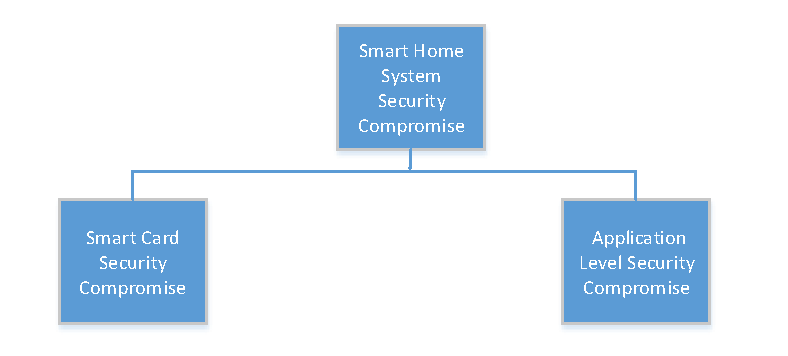
\includegraphics[width=0.85\textwidth]{attack-tree-overview}
		\caption{Attack Tree Overview}
	\label{fig:attack-tree-overview}
\end{figure}
As shown in figure~\ref{fig:attack-tree-overview} the attack tree is categorized into two main sub attack  trees. The first type group describes attacks that the third malicious party could apply to harm the smart card employed in my scenario. And the second one contains higher application level related threats, namely the security threats to the OPC UA standards and applications. 

\section{Smart Card Security Compromise}
In this section, I will firstly present the attack tree in the domain of smart card and based on this attack tree  perform the secure analysis. At last, countermeasures designed and integrated in my system are going to be described.

\subsection{Sub Attack Tree and its Content}
 \begin{figure}[!htb]
	\centering
	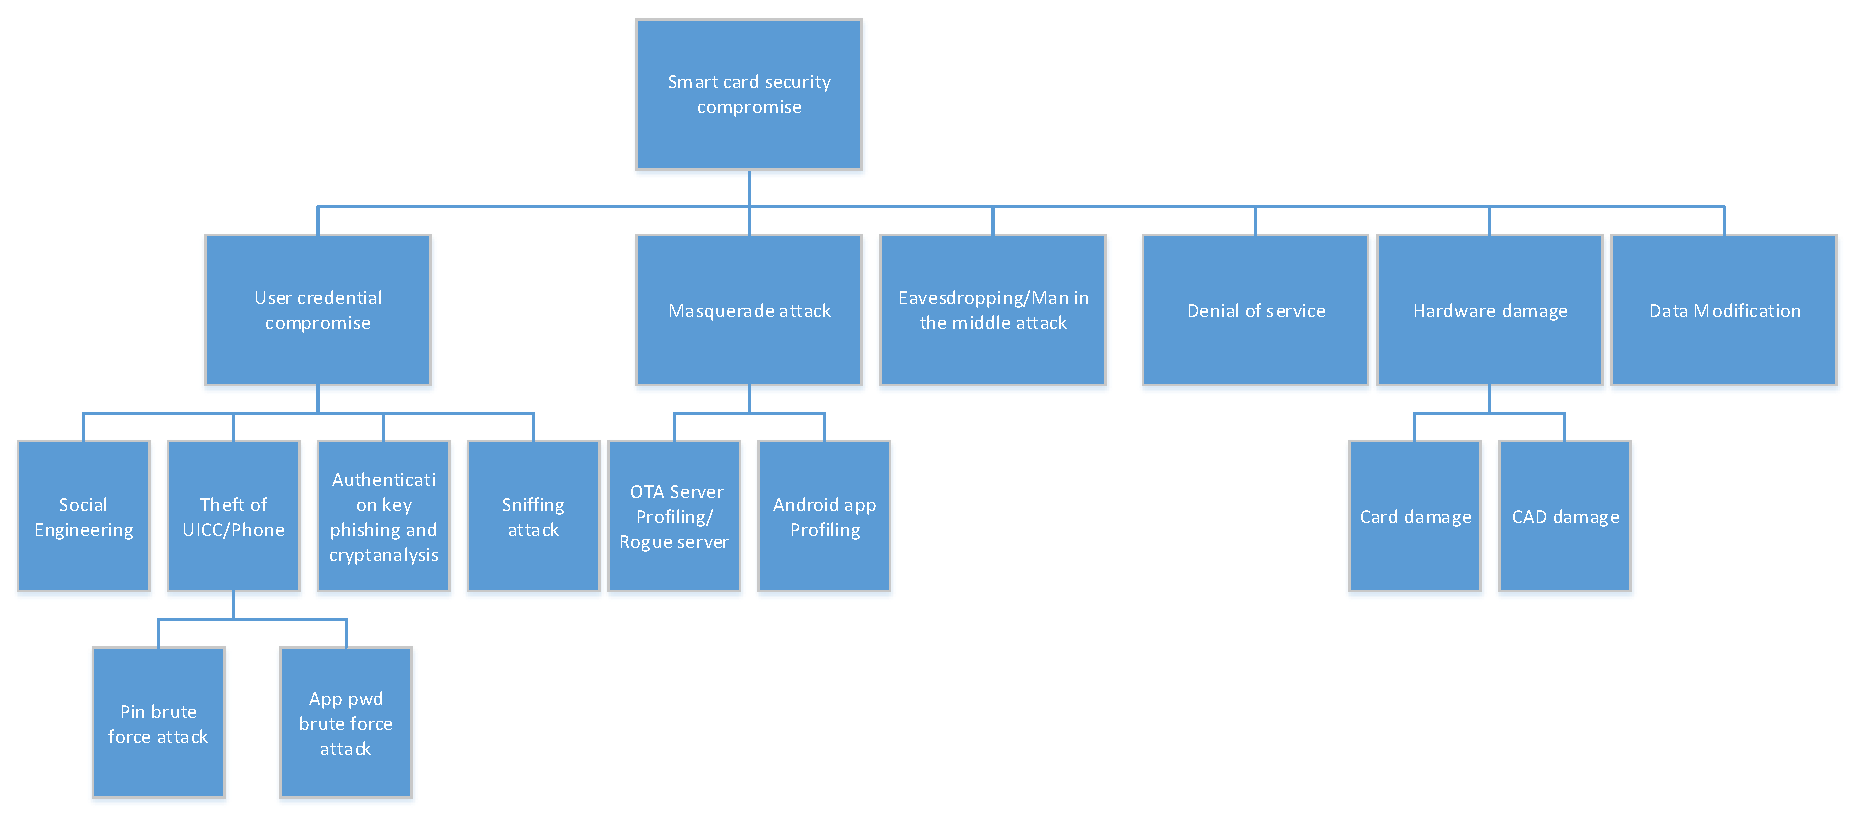
\includegraphics[width=1.0\textwidth]{attack-tree-smartcard}
		\caption{Smartcard Security Compromise}
	\label{fig:attack-tree-smartcard}
\end{figure}
Figure~\ref{fig:attack-tree-smartcard} illustrates the first category of potential threats. Since a number of attacks are listed in the figure which makes it hard to read detailed subcategories, therefore this sub attack tree is also presented as following,

\begin{enumerate}
	\item User credential compromise
  	\begin{enumerate}
    	\item Social Engineering
	\item Theft of UICC/Phone
		\begin{enumerate}
		\item Smart card PIN brute force attack
		\item Android Application password brute force attack
		\end{enumerate}
    	\item Authentication key phishing and cryptanalysis
    	\item Sniffing attack
	\end{enumerate}
	\item Masquerade attack
		\begin{enumerate}
		\item OTA server profiling/Rogue server
		\item Android application profiling
		\end{enumerate}
	\item Eavesdropping/Man in the middle attack
	\item Denial of service
	\item Hardware damage
		\begin{enumerate}
		\item Card  damage
		\item CAD damage
		\end{enumerate}
	\item  Data Modification
\end{enumerate}

\subsection{Analysis and Countermeasures}
Security mechanisms and countermeasures against potential threads to the smart card are described as following,
\begin{itemize}
\item \emph{against user credential compromise}. Any security system must have a human as the administrator or user, therefore the secure storage and usage of user credential shows its importance in the realm of computer security. As shown in the attack tree, following potential threads are presented,
\begin{itemize}
\item Social engineering, this attack refers to the process of psychological manipulation of user to for instance give out their password or to believe a fraud. In order to protect the end user, no one can get access to my system without the UICC smart card and the corresponding user password, which is used to unlock Android  application. In the worst case, which means, user gives his smart phone and password to the attacker, the system is also capable of recording any behaviors taking place during the period of fraud and providing forensic evidence.
\item Theft of phone or smart card. Even when the attacker manages to steal the smart phone, but without the acknowledge of the PIN and user password, which are used to unlock the smart card and Android application respectively, he can not get access to the system. Moreover both smart card and my Android application has the mechanism to block itself after three times of wrong input, which means brute force attack is not an option for the adversary.
\item Key phishing and cryptanalysis/ Sniffing. As introduced in section~\ref{labelKeyManagement}, smart card is the secure  credential  storage media and the keys used by smart card consist of various of information, such as key number, key indicator and so on. Consequently, even if the attacker has a segment of credential message, which is captured as a result of key phishing or sniffing, he can never figure out what encryption keys are applied without knowing the corresponding smart card key management system structure.
\end{itemize}
\item \emph{against masquerade attack.} In order to fraud the smart card and to get the credential information stored by it, the attacker could masquerade  himself as either the remote administrator server or the Android application designed by me.  But any of these two approaches will not work, because the smart card needs to perform TLS secure handshake before exchange any other information with the remote server as standardized by the \emph{GlobalPlatform}. Since fraud server can never pass the secure handshake, therefore the adversary is not able to get any useful information from smart card. Moreover if an Android application claims himself as the \emph{Smart Home App}, it must provide the corresponding application signature, as described in essential secure element  control protocols, which are also provided by the \emph{GloabalPlatform}. Since any fraud application is not capable of providing the correct application signature, this masquerade attack will not succeed. 
\item \emph{against eavesdropping and MitM attacks.} Since the communication between smart card and the remote server is session-based, even when an attacker is able to capture some communication messages, he still can't reply this message to the victim. 
\item \emph{against DoS attack..} The remote administrator server could be a victim of denial of service attack, when the adversary floods messages to the server and tries to harm the system. But the remote server applied in my scenario has the message exchanging rate control  mechanism, any partner that floods the message will be banned by the system for a period of time.
\item \emph{against Hardware damage.} Nowadays' smart cards are designed with the in section~\ref{secSMD} introduced protecting mechanisms against physical attacks, therefor attacks such as power difference analysis will not succeed. The major consequence of smart card hardware damage is that, users have to require a new card from the card provider and to bear the inconvenience brought by card damage. 
\item \emph{against data modification.} Data here refers not only to the information stored on the smart card but also the messages exchanged between smart card and the remote server.  As already introduced, smart card is a perfect storage media and independent of other external device. Moreover the exchanged messages are protected from the attacker by using checksum algorithm, which means any information modified by a third party is going to be ignored.
\end{itemize}

\section{OPC UA Application Level Security Compromise}
In this section, the second category of threads is discussed and corresponding countermeasures are presented.  
\subsection{Sub Attack Tree and its Content}
 \begin{figure}[!htb]
	\centering
	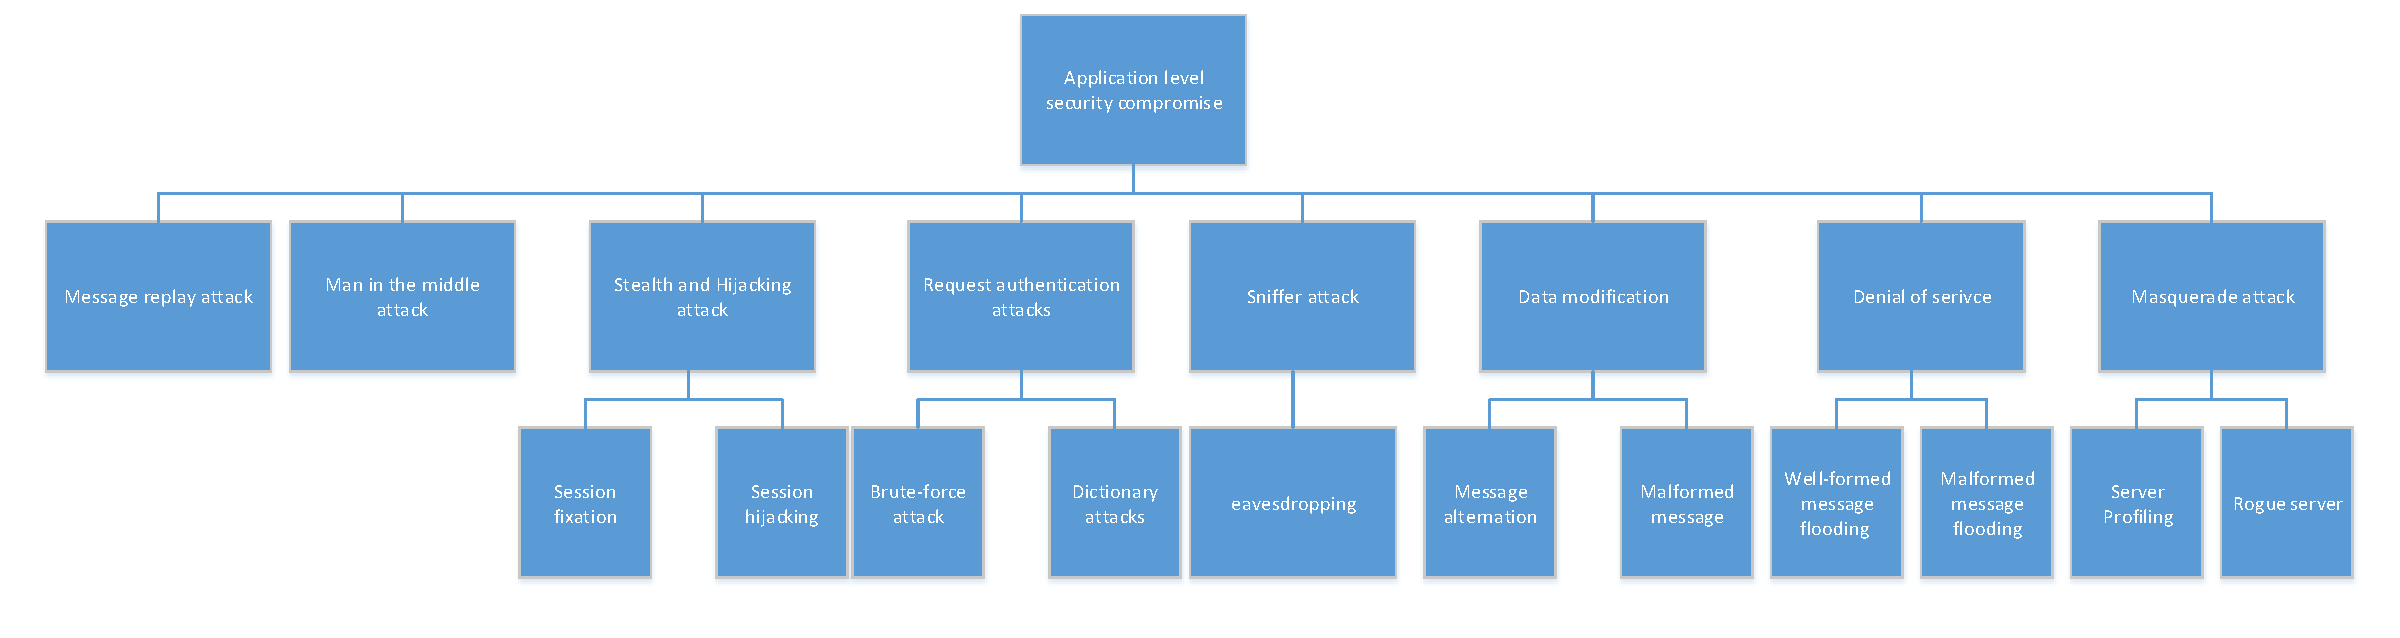
\includegraphics[width=1.0\textwidth]{attack-tree-application}
		\caption{OPC UA Application Security Compromise}
	\label{fig:attack-tree-application}
\end{figure}
The second category of threads which focus on the OPC UA application is pictured as figure~\ref{fig:attack-tree-application} and  the graph content is described as following,

\begin{enumerate}
	\item Message replay attack
	\item Man in the middle attack
	\item Stealth and Hijacking attack
  	\begin{enumerate}
    	\item Session fixation
	\item Session hijacking
	\end{enumerate}
		
    	\item Request authentication attacks
	\begin{enumerate}
		\item Brute-force attack
		\item Dictionary attacks
		\end{enumerate}
    	\item  Sniffing attack - eavesdropping

	\item Data modification
		\begin{enumerate}
		\item Message alternation
		\item Malformed message
		\end{enumerate}
	
	\item Denial of service
		\begin{enumerate}
		\item Well-formed message flooding
		\item Mal-formed message flooding
		\end{enumerate}

	\item Masquerade attack
		\begin{enumerate}
		\item Server profiling
		\item Rogues server
		\end{enumerate}
\end{enumerate}
\subsection{Analysis and Countermeasures}
In total eight categories of threads, which aim at the OPC UA client and server application code applied in my scenario, are analyzed. They are,

\begin{itemize}
\item \emph{Message replay attack and MitM attack.} Even when an adversary captures a message  exchanged for instance between housing device and smart phone, he can never successfully reply this message, because each request and response message is protected by its session ID, secure channel ID and alternatively sequence number.
\item \emph{Stealth and Hijacking attack.} In order to perform session hijacking attack, the attacker must firstly compromise the secure channel based on which the session is created. But the employed secure  channel is standardized by Globalplatform and protected with TLS handshake. Therefore this category of attack is prevented.
\item \emph{Request authentication attack.} No matter attacker applies brute force attack or dictionary attack, he only has three password or PIN input chances, which means it is extremely impossible for him to guess the authentication passwords or PIN.
\item \emph{Sniffing.} Encryption algorithms are always  applied in my system, therefore the adversary is not  able to understand  the message he sniffed and the system confidentiality is protected.
\item \emph{Data modification.} Both symmetric and asymmetric signatures are employed in OPC UA standards, any by third party illegitimately modified message can not pass the signature examination test and will be ignored.
\item \emph{Denial of service.} In order to protect  the service availability of my system, the message  exchanging rate is controlled. 
\item \emph{Masquerade attack.} Masquerade attacks are impossible in my system for the following reasons. Firstly if a malicious application claims itself to be a OPC UA client or server partner, it must provide necessary secure information such as secure keys and certificates before performing any other actions. Moreover, the adversary also has to be able to perform dual authentication with the remote administrator server. Even when the fraud application manages to receive a message, it doesn't possess the required  private keys to decrypt the content. 
\end{itemize}

\section{Conclusion}
In conclusion, my proposal system is strong against the known attacks presented in the above pictured attack tree by adopting the combination of the magic bullet - smart card and the newly released OPC UA specifications. 
